\documentclass[a4paper, 12pt]{article}%тип документа

%отступы
\usepackage[left=2cm,right=2cm,top=2cm,bottom=3cm,bindingoffset=0cm]{geometry}
\setlength{\parindent}{5ex}

%Русский язык
\usepackage[T2A]{fontenc} %кодировка
\usepackage[utf8]{inputenc} %кодировка исходного кода
\usepackage[english,russian]{babel} %локализация и переносы

%Вставка картинок
\usepackage{graphicx}
\graphicspath{{pictures/}}
\DeclareGraphicsExtensions{.pdf,.png,.jpg}

%Графики
\usepackage{pgfplots}
\pgfplotsset{compat=1.9}

%Математика
\usepackage{amsmath, amsfonts, amssymb, amsthm, mathtools}

%Таблицы
\usepackage{longtable} 
\usepackage{float}

%Римские цифры
\newcommand{\RomanNumeralCaps}[1]{\uppercase\expandafter{\romannumeral#1}}

\usepackage{multirow}


\begin{document}
	\begin{titlepage}
		\begin{center}
			\textsc{Федеральное государственное автономное образовательное учреждение высшего образования«Московский физико-технический институт (национальный исследовательский университет)»\\[5mm]
			}
			
			\vfill
			
			\textbf{Отчёт по лабораторной работы 1.4.5\\[3mm]
				Изучение колебаний струны.
				\\[50mm]
			}
			
		\end{center}
		
		\hfill
		\begin{minipage}{.5\textwidth}
			Выполнил студент:\\[2mm]
			Сериков Василий Романович\\[2mm]
			группа: Б03-102\\[5mm]
			
		\end{minipage}
		\vfill
		\begin{center}
			Москва, 2021 г.
		\end{center}
		
	\end{titlepage}
	
	\newpage
	\textbf{Цель работы:} изучить поперечные стоячие волны на тонкой натянутой струне;
	измерить собственные частоты колебаний струны и проверить условие образования
	стоячих волн; измерить скорость распространения поперечных волн на струне и исследовать её зависимость от натяжения струны. \\
	
	\textbf{В работе используется:} закрепленная на станине стальная струна, набор грузов, электромагнитные датчики, звуковой генератор, двухканальный осциллограф,
	частотомер. \\
	
	\textbf{Теория:} Струной в акустике называют однородную тонкую гибкую упругую
	нить. Примерами могут служить сильно натянутый шнур или трос, струны
	гитары, скрипки и других музыкальных инструментов. В данной работе
	изучаются поперечные колебания стальной гитарной струны, натянутой горизонтально и закрепленной между двумя неподвижными зажимами.
	Основное свойство струны — гибкость — обусловлено тем, что её поперечные размеры малы по сравнению с длиной. Это означает, что напряжение в струне может быть направлено только вдоль неё, и позволяет не
	учитывать изгибные напряжения, которые могли бы возникать при поперечных деформациях (то есть при изгибе струны)\\
	
	Второй закон Ньютона для вертикального движения элемента струны запишется в следующем виде: 
	$$\delta_m \frac{\partial^2 y}{\partial t^2} - T_1 \sin{\alpha_1} - T_2\sin{\alpha_2} $$

	Основываясь на предположении, что отклонения струны от положения
	равновесия малы, можем сделать ряд упрощений:\\ 
	1. Длина участка струны в смещенном состоянии практически равна
	длине участка в положении равновесия * , поэтому добавочным
	напряжением вследствие удлинения струны при деформации можно пренебречь. Следовательно, силы $T_1$ и $T_2$ по модулю равны силе
	натяжения струны: $T_1 \approx T_2 \approx T$.\\ 
	2. Углы наклона $\alpha$ малы, поэтому $\tan{\alpha} \approx \sin{\alpha} \approx \alpha$, и, следовательно,
	можно положить $\alpha \approx \frac{\partial y}{\partial x}$\\
	
	Тогда волновое уравнение примет вид:
	$$ \frac{\partial^2 y}{\partial t^2} = u^2 \frac{\partial^2 y}{\partial x^2}, 	           \text{где  }  u = \sqrt{\frac{T}{\rho_l}} $$
	
	Стоячие волны на струне с закреплёнными концами образуются, только если на длине струны укладывается целое число полуволн: $ \lambda_n = \frac {2L}{n} $
	
	Поскольку длина волны однозначно связана с её частотой, струна может
	колебаться только с определёнными частотами: $\nu_n = \frac{n}{2L} \sqrt{\frac{T}{\rho_l}}$

	\begin{figure}[h]
		\center{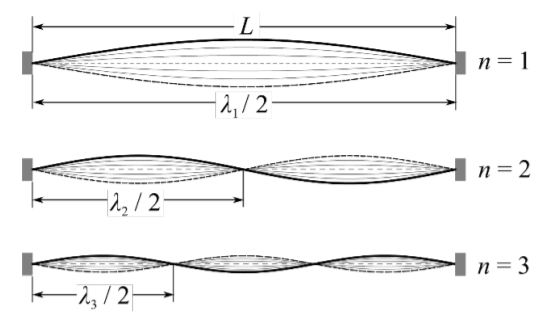
\includegraphics [scale=1]{str.png}}
		\caption{Стоячие волны (собственные моды колебаний струны) для n = 1, 2, 3}
	\end{figure}
    \begin{figure}[H]
      	\center{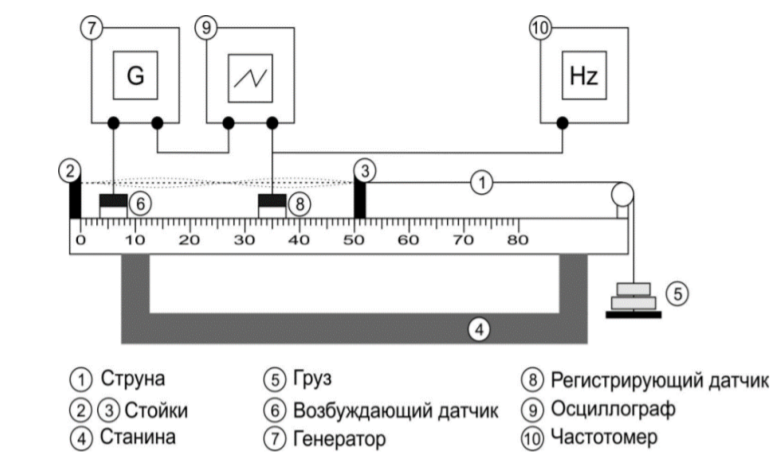
\includegraphics [scale=1]{ust.png}}
    	\caption{ Экспериментальная установка}
    \end{figure}

    \newpage
    \textbf{Ход работы:}
    \begin{enumerate}
	\item  Проведем  предварительные расчёты. Оценим скорость распространения волны u по формуле: $u=\sqrt{\frac{T}{\rho_l}} $,  где T = 12,3 Н, $\rho_l = 568,4 $ мг/м,  Тогда $u = 151$ м/с.
	
	Также рассчитаем частоту основной гармоники $\nu_1$ по формуле: $\nu_n = \frac{n}{2L} \sqrt{\frac{T}{\rho_l}}$,\\
	 $\sigma{\nu_n}=\nu_n \frac{\sigma_L}{L}$, L=50,0$\pm$0,1 см.
	 	
	 $\nu_1 = (15,1 \pm 0,1)*10$ Гц
	 
	 
	 
	 \item Запишите значения частот $\nu_n$ стоячих волн, которые удастся пронаблюдать, изменяя частоту генератора.
	 
	 	\begin{longtable}{|c|c|}
	 		\hline 
	 		n & $\nu$, Гц \\
	 		\hline
	 		1 & 151,2 \\
	 		\hline
	 		2 & 306,5 \\
	 		\hline
	 		3 & 453, 6 \\
	 		\hline
	 		4 & 604,8 \\
	 		\hline
	 		5 & 756,0\\
	 		\hline
	 		\caption{Частоты наблюдаемых стоячих волн}
	 	\end{longtable}
 	

     \item Проведем измерения частот для четных и нечетных гармоник стоячих волн при разных натяжениях струны. Данные занесем в таблицы 2-6. Погрешность измерения частоты данным способом имеет значение $\sigma{\nu_n}=\pm 1$ Гц, данное значение получено экспериментально.
     
     
     	\begin{minipage}{0.4\textwidth}
     	\begin{longtable}{|c|c|}
     		\hline 
     		n & $\nu$, Гц \\
     		\hline
     		1 & 181\\
     		\hline
     		2 & 365\\
     		\hline
     		3 & 549\\
     		\hline
     		4 & 733\\
     		\hline
     		5 & 906\\
     		\hline
     		6 & 1095\\
     		\hline
     		7 & 1273\\
     		\hline
     		8 & 1467\\
     		\hline
     		9 & 1636\\
     		\hline
     		\caption{Частоты при  T=17,1 Н}
     	\end{longtable}
     \end{minipage} 
 	\begin{minipage}{0.4\textwidth}
 	\begin{longtable}{|c|c|}
 		\hline 
 		n & $\nu$, Гц \\
 		\hline
 		1 & 205\\
 		\hline
 		2 & 412\\
 		\hline
 		3 & 619\\
 		\hline
 		4 & 824\\
 		\hline
 		5 & 1030\\
 		\hline
 		6 & 1238\\
 		\hline
 		7 & 1444\\
 		\hline
 		8 & 1655\\
 		\hline
 		9 & 1861\\
 		\hline
 		\caption{Частоты при T=21,9 Н}
 	\end{longtable}
 \end{minipage}
\\
	\begin{minipage}{0.4\textwidth}
	\begin{longtable}{|c|c|}
		\hline 
		n & $\nu$, Гц \\
		\hline
		1 & 229\\
		\hline
		2 & 460\\
		\hline
		3 & 687\\
		\hline
		4 & 940\\
		\hline
		5 & 1147\\
		\hline
		6 & 1379\\
		\hline
		7 & 1609\\
		\hline
		8 & 1843\\
		\hline
		9 & 2075\\
		\hline
		\caption{Частоты при T=26,8 Н}
	\end{longtable}
\end{minipage}
    	\begin{minipage}{0.4\textwidth}
    	\begin{longtable}{|c|c|}
    		\hline 
    		n & $\nu$, Гц \\
    		\hline
    		1 & 249\\
    		\hline
    		2 & 499\\
    		\hline
    		3 & 746\\
    		\hline
    		4 & 996\\
    		\hline
    		5 & 1244\\
    		\hline
    		6 & 1492\\
    		\hline
    		7 & 1745\\
    		\hline
    		8 & 1993\\
    		\hline
    		9 & 2249\\
    		\hline
    		\caption{Частоты при T=31,7 Н}
    	\end{longtable}
    \end{minipage}
     \\
     	\begin{longtable}{|c|c|}
     		\hline 
     		n & $\nu$, Гц \\
     		\hline
     		1 & 262\\
     		\hline
     		2 & 524\\
     		\hline
     		3 & 786\\
     		\hline
     		4 & 1048\\
     		\hline
     		5 & 1312\\
     		\hline
     		6 & 1575\\
     		\hline
     		7 & 1837\\
     		\hline
     		8 & 2099\\
     		\hline
     		9 & 2366\\
     		\hline
     		\caption{Частоты при T=35 Н}
     	\end{longtable}
     
     \item Построим график (Рис.3) зависимости частоты от номера гармоники для 5 натяжений проволоки.
     
  \begin{figure}[H]
\center{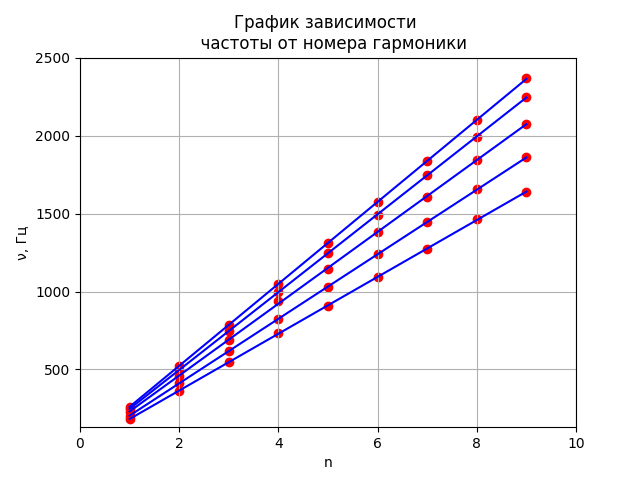
\includegraphics [scale=0.7]{first6.png}}
\caption{}
\end{figure}

\newpage
\item Вычислим скорость волн u по наклону прямой по МНК, также вычислим погрешность. Результаты занесем в таблицу 7.
  
  \begin{longtable}{|c|c|c|c|c|c|}
  	\hline 
  	u м/с & 173& 196& 218& 237& 248\\
  	\hline
  	$\sigma_u$ м/с &2 &2&2&3&3\\
  	\hline
  	\caption{Значения скорости волн}
  \end{longtable}

\item Построим график (Рис.4) зависимости квадрата скорости волны $u^2$ от силы натяжения T.
\begin{figure}[H]
	\center{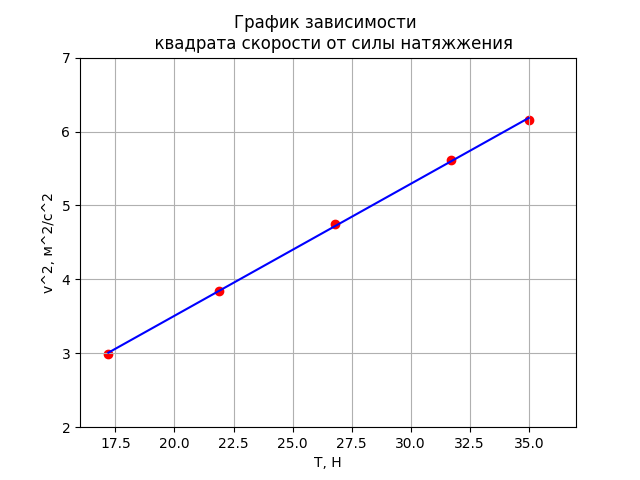
\includegraphics [scale=0.7]{first7.png}}
	\caption{}
\end{figure}

\item По наклону прямой определим погонную плотность, также определим значение погрешности по МНК. $\rho_l=(56,1\pm 0,8)*10^{-5}$ кг/м. Полученное нами значение погонной плотности совпадает в пределах погрешности со значением указанным на установке (568,4 мг/м).

\item Благодаря высокой добротности струны, возможно возбуждение её
колебаний при кратных частотах генератора, меньших, чем $\nu_1$. Уменьшим частоту на генераторе до значения $\nu=\nu_1 /2$. На осциллографе получим фигуру Лиссажу с одном самопересечением(Рис.5). Полученная фигура имеет одну точку самопересечения, так как настроенная частота отличается от резонансной в 2 раза.


\begin{figure}[H]
	\center{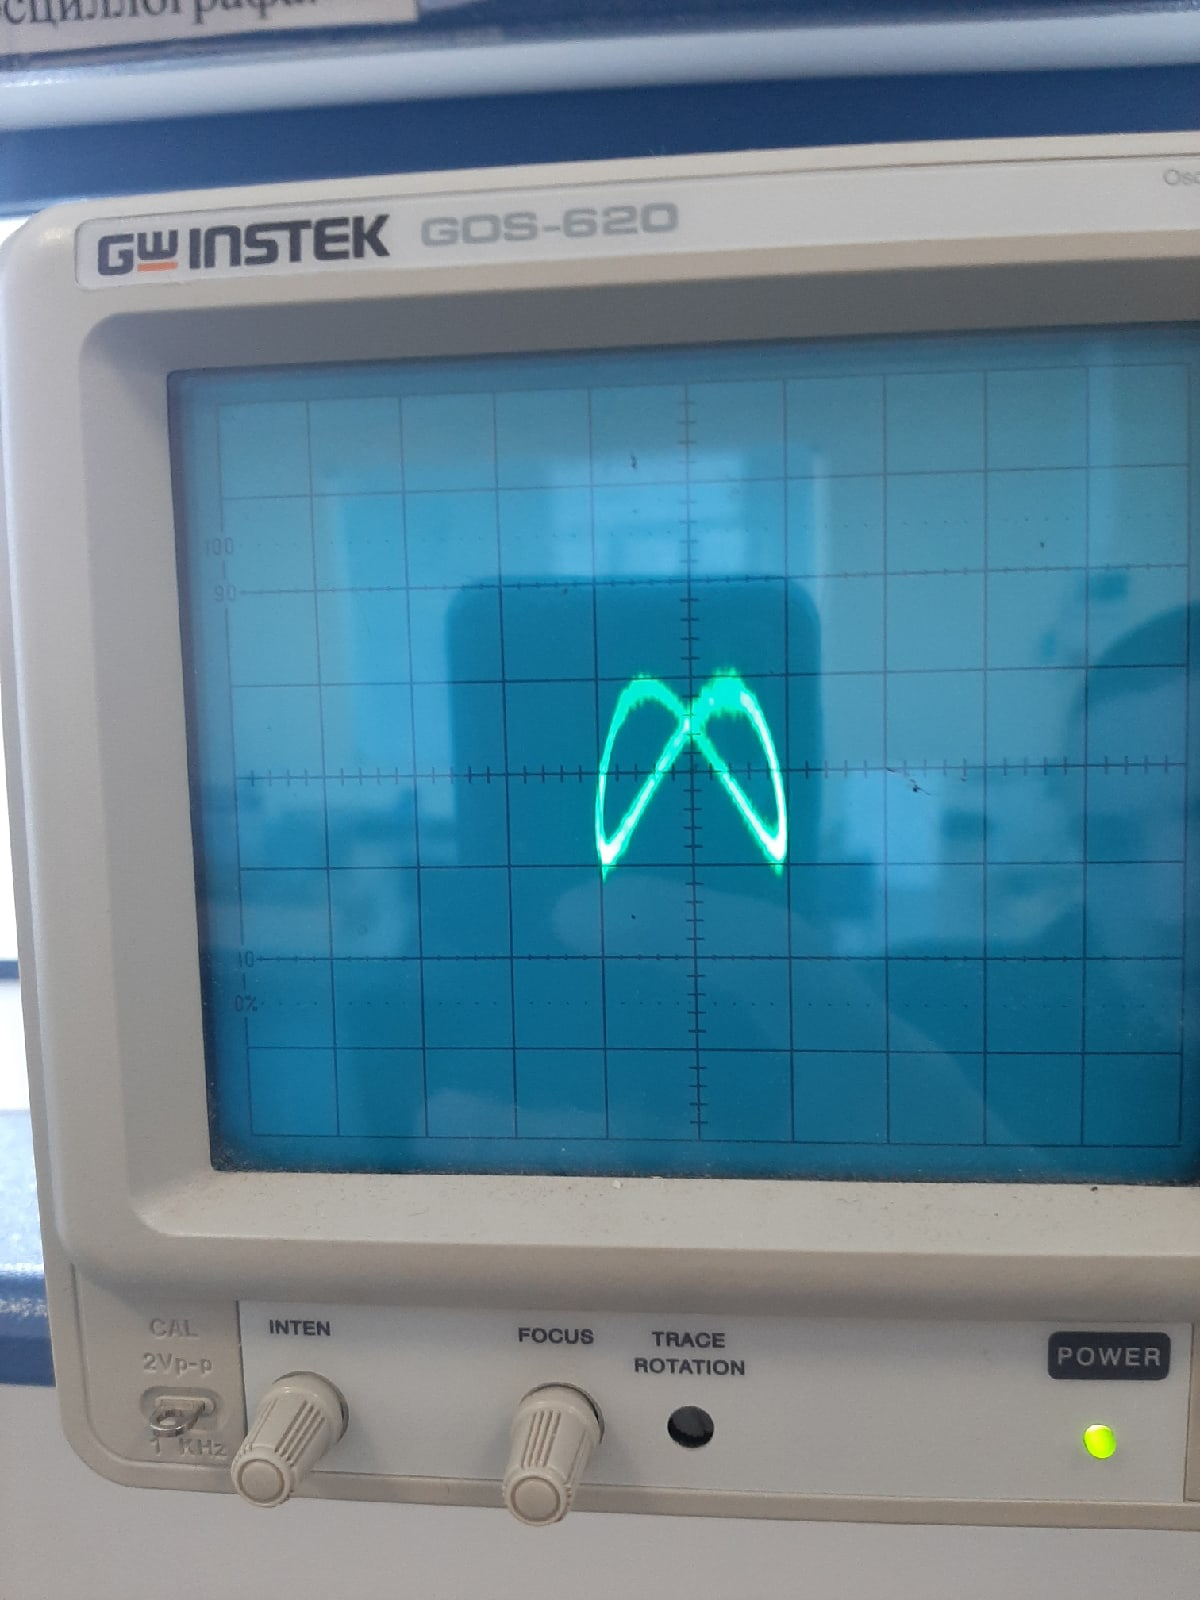
\includegraphics [scale=0.3]{liss.jpg}}
	\caption{}
\end{figure}
  \textbf{Вывод:} : В данной работе мы изучили поперечные стоячие волн на тонкой натянутой струне, измерили собственные частоты колебаний струны, измерили скорость распространения поперечных волн на струне и исследовали её зависимость от натяжения струны. По полученным данным построили  графики.


\end{enumerate}
\end{document}